\subsection{External Interface Requirements}
\subsection{Performance Requirements}
\subsection{Design Constraints}
\begin{enumerate}
	\item Query caching
	\newline
	In order to avoid traffic requests to the database and to speed up database , query caching is crucial. AdoDB provides powerful caching system which can implemented in the navUP system and help improve speed regarding interaction between front end and database.
\end{enumerate}
\subsection{Software System Attributes}
\subsection{UML diagrams}
\subsubsection{Activity diagram}
\begin{figure}[H]
	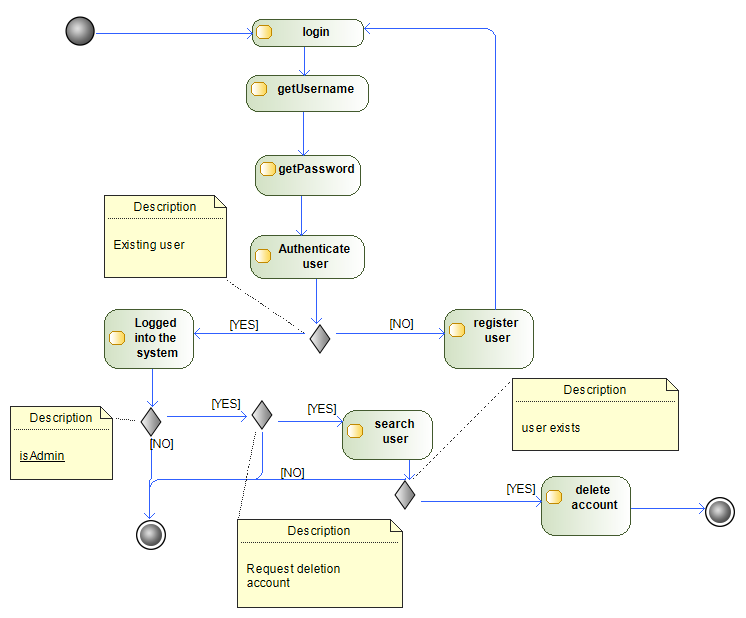
\includegraphics[width=12cm,height=26cm,keepaspectratio]{Users/Pictures/user_Activity_diagram.png}
	\caption{Activity diagram for user management module}\label{visina8}
\end{figure}
\subsubsection{Use Case diagram}
\begin{figure}[H]
	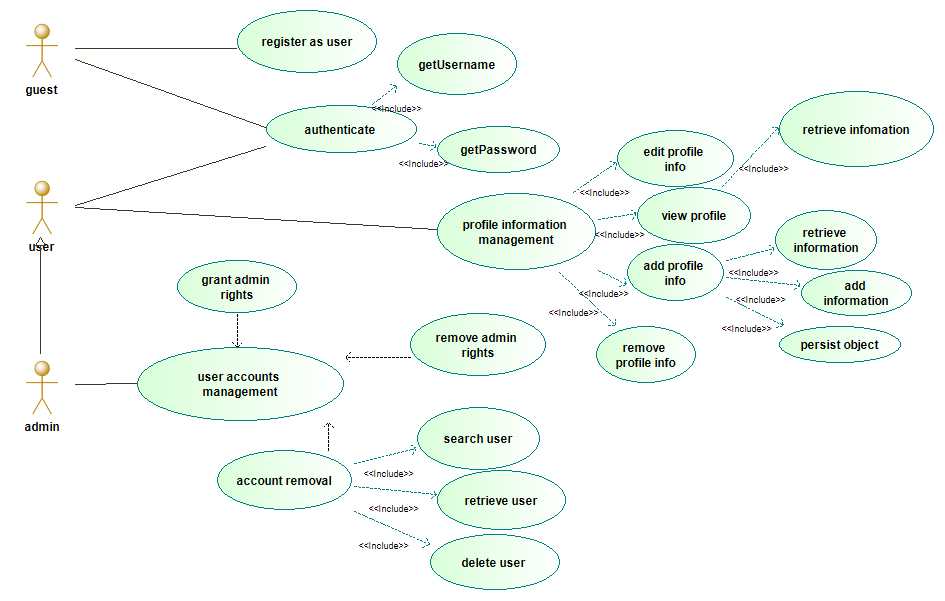
\includegraphics[width=12cm,height=26cm,keepaspectratio]{Users/Pictures/user_use_case_diagram.png}
	\caption{Use case diagram for user management module}\label{visina8}
\end{figure}
